\section{Ideal Prediction, Bayes Rules, and Learnable Models}

The previous section introduced expected risk as the population-level objective of learning. Once that objective is in place, a natural question appears immediately:

\begin{quote}
If the true data-generating distribution were known, what prediction rule would be optimal under a chosen loss?
\end{quote}

This question leads to one of the central reference objects of statistical learning: the \emph{Bayes-optimal predictor}. It is an ideal object rather than a practically available one, but it gives the benchmark against which all real learning procedures should be compared.

\subsection*{Bayes-optimal prediction as conditional optimization}

Let $\ell(\hat y,y)$ be a loss function, and let
\[
R(f)=\mathbb E[\ell(f(X),Y)]
\]
denote the expected risk of a predictor $f$.

\begin{definition}[Bayes-optimal predictor]
A predictor $f^\star$ is called \emph{Bayes-optimal} if it minimizes expected risk over all measurable predictors:
\[
f^\star \in \arg\min_f R(f).
\]
The corresponding minimum value
\[
R^\star = R(f^\star)
\]
is called the \emph{Bayes risk}.
\end{definition}

The key idea is that expected risk can be analyzed conditionally on the input. For each fixed input value $x$ and each candidate action $a$, define the conditional risk
\[
L_x(a)=\mathbb E[\ell(a,Y)\mid X=x].
\]
This turns the global optimization problem over functions into a family of local decision problems, one for each input value.

\begin{theorem}[Pointwise conditional minimization yields global risk minimization]
Assume there exists a measurable predictor $f^\star$ such that for almost every $x$,
\[
f^\star(x)\in \arg\min_a \mathbb E[\ell(a,Y)\mid X=x].
\]
Then $f^\star$ is Bayes-optimal. Moreover, for every predictor $f$,
\[
R(f)-R(f^\star)
=
\mathbb E\!\left[
\mathbb E[\ell(f(X),Y)\mid X]
-
\mathbb E[\ell(f^\star(X),Y)\mid X]
\right]
\ge 0.
\]
\end{theorem}

\begin{proof}
For any predictor $f$, the tower property of conditional expectation gives
\[
R(f)=\mathbb E[\ell(f(X),Y)]
=
\mathbb E\!\left[\mathbb E[\ell(f(X),Y)\mid X]\right].
\]
Likewise,
\[
R(f^\star)=
\mathbb E\!\left[\mathbb E[\ell(f^\star(X),Y)\mid X]\right].
\]
Hence
\[
R(f)-R(f^\star)
=
\mathbb E\!\left[
\mathbb E[\ell(f(X),Y)\mid X]
-
\mathbb E[\ell(f^\star(X),Y)\mid X]
\right].
\]
Now fix a realized value $X=x$. By assumption, $f^\star(x)$ minimizes
\[
a\mapsto \mathbb E[\ell(a,Y)\mid X=x].
\]
Therefore,
\[
\mathbb E[\ell(f(x),Y)\mid X=x]
\ge
\mathbb E[\ell(f^\star(x),Y)\mid X=x]
\]
for almost every $x$. Taking expectation over $X$ yields
\[
R(f)\ge R(f^\star).
\]
Thus $f^\star$ is Bayes-optimal.
\end{proof}

This theorem is one of the fundamental structural results in learning theory. It says that optimal prediction is governed by the conditional law of $Y$ given $X=x$. To understand ideal prediction, one studies
\[
P(Y\mid X=x).
\]

\begin{figure}[tbp]
\centering
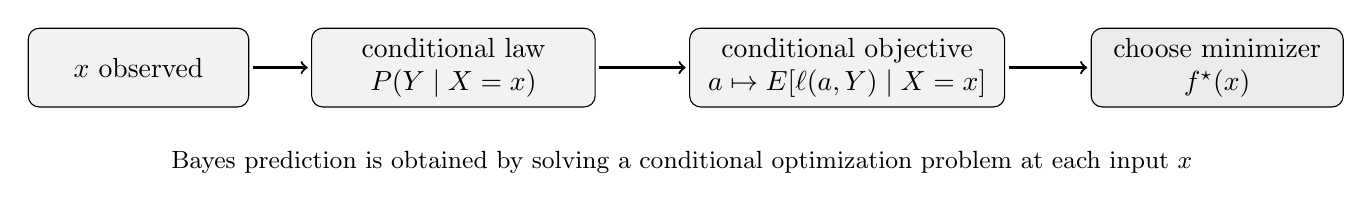
\begin{tikzpicture}[scale=1, every node/.style={align=center}]
    \node[draw, rounded corners, fill=gray!10, minimum width=2.8cm, minimum height=1cm] (x) at (0,0) {$x$ observed};
    \node[draw, rounded corners, fill=gray!10, minimum width=3.6cm, minimum height=1cm] (cond) at (4,0) {conditional law\\$P(Y\mid X=x)$};
    \node[draw, rounded corners, fill=gray!10, minimum width=4cm, minimum height=1cm] (risk) at (9,0) {conditional objective\\$a\mapsto \mathbb E[\ell(a,Y)\mid X=x]$};
    \node[draw, rounded corners, fill=gray!15, minimum width=3.2cm, minimum height=1cm] (bayes) at (13.7,0) {choose minimizer\\$f^\star(x)$};

    \draw[->, thick] (1.45,0) -- (2.15,0);
    \draw[->, thick] (5.85,0) -- (6.95,0);
    \draw[->, thick] (11.05,0) -- (12.05,0);

    \node at (6.9,-1.2) {\small Bayes prediction is obtained by solving a conditional optimization problem at each input $x$};
\end{tikzpicture}
\caption{The Bayes decision rule: once $x$ is observed, the conditional distribution $P(Y\mid X=x)$ determines the conditional risk for each candidate action $a$, and the optimal choice is the minimizer of that conditional risk.}
\end{figure}

\subsection*{Squared loss and the conditional mean}

Suppose $\mathcal Y=\mathbb R$ and consider squared loss
\[
\ell(\hat y,y)=(\hat y-y)^2.
\]

\begin{proposition}[Bayes predictor under squared loss]
Under squared loss, any Bayes-optimal predictor is given by the conditional mean:
\[
f^\star(x)=\mathbb E[Y\mid X=x].
\]
\end{proposition}

\begin{proof}
Fix $x$ and let
\[
m(x)=\mathbb E[Y\mid X=x].
\]
For any candidate prediction $a$,
\[
a-Y=(a-m(x))+(m(x)-Y),
\]
so
\[
(a-Y)^2
=
(a-m(x))^2
+
2(a-m(x))(m(x)-Y)
+
(m(x)-Y)^2.
\]
Taking conditional expectation given $X=x$,
\[
\mathbb E[(a-Y)^2\mid X=x]
=
(a-m(x))^2
+
2(a-m(x))\mathbb E[m(x)-Y\mid X=x]
+
\mathbb E[(m(x)-Y)^2\mid X=x].
\]
Because
\[
\mathbb E[m(x)-Y\mid X=x]
=
m(x)-\mathbb E[Y\mid X=x]
=
0,
\]
this becomes
\[
\mathbb E[(a-Y)^2\mid X=x]
=
(a-m(x))^2+\mathbb E[(m(x)-Y)^2\mid X=x].
\]
The second term does not depend on $a$, so the minimum is attained at
\[
a=m(x)=\mathbb E[Y\mid X=x].
\]
The theorem above then implies that the Bayes-optimal predictor is
\[
f^\star(x)=\mathbb E[Y\mid X=x].
\qedhere
\]
\end{proof}

Thus regression under squared loss is fundamentally about estimating a conditional expectation.

\subsection*{Absolute loss and the conditional median}

Now consider absolute loss
\[
\ell(\hat y,y)=|\hat y-y|.
\]

\begin{proposition}[Bayes predictor under absolute loss]
Under absolute loss, any Bayes-optimal predictor is a conditional median:
\[
f^\star(x)\in \mathrm{Median}(Y\mid X=x).
\]
More precisely, a value $a$ is optimal at $x$ if
\[
\mathbb P(Y\le a\mid X=x)\ge \frac12
\qquad\text{and}\qquad
\mathbb P(Y\ge a\mid X=x)\ge \frac12.
\]
\end{proposition}

\begin{proof}[Proof sketch]
Fix $x$ and define
\[
\phi_x(a)=\mathbb E[|a-Y|\mid X=x].
\]
If $a$ is moved slightly to the right, the loss decreases for outcomes with $Y>a$ and increases for outcomes with $Y<a$. The optimum therefore occurs when the conditional mass on the two sides is balanced. More formally, the one-sided derivatives satisfy
\[
\phi_x'(a^-)=\mathbb P(Y<a\mid X=x)-\mathbb P(Y\ge a\mid X=x),
\]
\[
\phi_x'(a^+)=\mathbb P(Y\le a\mid X=x)-\mathbb P(Y>a\mid X=x),
\]
so $a$ minimizes $\phi_x$ exactly when
\[
\phi_x'(a^-)\le 0 \le \phi_x'(a^+),
\]
which is equivalent to the stated median conditions.
\end{proof}

Under absolute loss, the ideal prediction is not the conditional mean in general. Different losses produce different notions of optimal prediction.

\subsection*{Zero--one loss and the Bayes classifier}

Now suppose the output space is a finite label set $\mathcal Y$ and the loss is zero--one loss,
\[
\ell(\hat y,y)=\mathbf 1\{\hat y\neq y\}.
\]

\begin{proposition}[Bayes classifier under zero--one loss]
Under zero--one loss, a Bayes-optimal classifier is given by
\[
f^\star(x)\in \arg\max_{y\in\mathcal Y} \mathbb P(Y=y\mid X=x).
\]
\end{proposition}

\begin{proof}
Fix $x$ and predict class $c\in\mathcal Y$. The conditional risk is
\[
\mathbb E[\mathbf 1\{c\neq Y\}\mid X=x]
=
\mathbb P(Y\neq c\mid X=x)
=
1-\mathbb P(Y=c\mid X=x).
\]
Minimizing this over $c$ is equivalent to maximizing
\[
\mathbb P(Y=c\mid X=x).
\]
Applying the theorem on pointwise conditional minimization completes the proof.
\end{proof}

This is often called the \emph{maximum a posteriori} rule, or MAP rule.

\subsection*{A worked example: binary posterior and decision threshold}

Consider binary classification with labels $\mathcal Y=\{0,1\}$. Suppose that for a given input $x$, the posterior probabilities are
\[
\mathbb P(Y=1\mid X=x)=0.73,
\qquad
\mathbb P(Y=0\mid X=x)=0.27.
\]
Under zero--one loss, the conditional risks of the two possible predictions are
\[
L_x(1)=\mathbb P(Y\neq 1\mid X=x)=0.27,
\]
\[
L_x(0)=\mathbb P(Y\neq 0\mid X=x)=0.73.
\]
Hence the Bayes classifier chooses class $1$.

More generally, in binary classification under zero--one loss, the Bayes rule is
\[
f^\star(x)=
\begin{cases}
1, & \text{if } \mathbb P(Y=1\mid X=x)\ge \frac12,\\[4pt]
0, & \text{if } \mathbb P(Y=1\mid X=x)< \frac12.
\end{cases}
\]
Thus the familiar threshold $1/2$ is not arbitrary; it arises from minimizing conditional misclassification probability.

\subsection*{Bayes risk and irreducible uncertainty}

Even the Bayes-optimal predictor is generally not perfect. The minimum possible expected risk
\[
R^\star=R(f^\star)
\]
is the error level forced by the data-generating process itself under the chosen loss.

For squared loss, the proof above shows that the minimum conditional risk at input $x$ is
\[
\mathbb E\!\left[(Y-\mathbb E[Y\mid X=x])^2 \mid X=x\right]
=
\mathrm{Var}(Y\mid X=x),
\]
so the Bayes risk is
\[
R^\star=\mathbb E[\mathrm{Var}(Y\mid X)].
\]
This is the part of the error that remains even when the conditional mean is known exactly.

For classification under zero--one loss, the minimum conditional error at $x$ is
\[
1-\max_{y\in\mathcal Y}\mathbb P(Y=y\mid X=x).
\]
If two labels both have positive conditional probability at the same $x$, then no deterministic classifier can always be correct there.

So Bayes-optimal does not mean error-free. It means only that no other predictor can do better on average under the specified loss.

\commonconfusion{Bayes-optimal does not mean computable. The Bayes rule is defined in terms of the true conditional distribution $P(Y\mid X=x)$, which is not known to the learner. It is an ideal benchmark, not usually an algorithm. Real learning methods use finite data to approximate this benchmark within restricted model classes.}

\subsection*{From ideal prediction to learnable models}

The Bayes rule is the best conceivable predictor relative to the true distribution and the chosen loss. But practical learning takes place under much stronger constraints:

\begin{itemize}
    \item the distribution $P$ is unknown,
    \item only a finite sample is available,
    \item computation is limited,
    \item the learner works within a restricted hypothesis class $\mathcal H$.
\end{itemize}

Thus real learning usually cannot search over all measurable predictors. Instead, it seeks a predictor
\[
\hat f \in \mathcal H
\]
that performs well relative to the Bayes benchmark. This leads naturally to the best-in-class predictor
\[
f_{\mathcal H}^\star \in \arg\min_{f\in\mathcal H} R(f),
\]
which need not coincide with the Bayes-optimal predictor $f^\star$.

The central tension is therefore clear:

\begin{quote}
The Bayes rule tells us what ideal prediction would be. Learning theory asks when finite data and restricted models allow us to approach that ideal.
\end{quote}

That tension drives the rest of the chapter.

\whattoremember{The Bayes-optimal predictor minimizes expected risk, and it is obtained by minimizing conditional risk pointwise at each input $x$. Under squared loss, the Bayes predictor is the conditional mean; under absolute loss, it is a conditional median; under zero--one loss, it is the most probable class given $x$. The Bayes rule is a benchmark determined by the true conditional law $P(Y\mid X=x)$, not something we usually know or can compute directly.}

\subsection*{Exercises}

\begin{exercise}
Let $\ell(\hat y,y)=(\hat y-y)^2$. Starting from
\[
\mathbb E[(a-Y)^2\mid X=x],
\]
show directly that the minimizing value of $a$ is $\mathbb E[Y\mid X=x]$.
\end{exercise}

\begin{exercise}
Suppose $\mathbb P(Y=1\mid X=x)=p(x)$ in a binary classification problem. Under zero--one loss, write down the Bayes classifier explicitly and explain why the threshold is $1/2$.
\end{exercise}

\begin{exercise}
Give an example of two different loss functions that would lead to two different notions of ideal prediction for the same conditional distribution of $Y\mid X=x$.
\end{exercise}

\begin{exercise}
Explain in words why Bayes-optimal prediction is a useful theoretical benchmark even though the learner does not know the true distribution.
\end{exercise}

\begin{exercise}
Suppose a regression problem satisfies
\[
Y = g(X)+\varepsilon,
\qquad
\mathbb E[\varepsilon\mid X]=0.
\]
Show that under squared loss the Bayes-optimal predictor is $g(X)$.
\end{exercise}

\begin{exercise}
For a three-class problem, suppose that at some input $x$,
\[
\mathbb P(Y=1\mid X=x)=0.4,\qquad
\mathbb P(Y=2\mid X=x)=0.35,\qquad
\mathbb P(Y=3\mid X=x)=0.25.
\]
What is the Bayes-optimal prediction under zero--one loss, and what is the corresponding conditional Bayes error?
\end{exercise}

\subsection*{Notes and references}

This section introduces one of the most important ideal objects in statistical learning: the Bayes-optimal predictor. Its role is conceptual and mathematical. Conceptual, because it makes clear that learning aims to approximate conditional structure rather than merely fit a sample. Mathematical, because it links prediction to the conditional distribution $P(Y\mid X=x)$ and shows that different losses induce different notions of optimal prediction. The Bayes benchmark will reappear later when we study generalization, approximation, model classes, and the limits of finite-sample learning.